% =================================================
% CAPITOLO 7 – Test Sperimentali e Analisi dei Risultati
% =================================================

\chapter{Test Sperimentali e Analisi dei Risultati}

\section{Setup Sperimentale}

I test sono stati condotti su una sequenza video acquisita a mano libera con movimento di avanzamento (camminata) e oscillazioni verticali periodiche dovute ai passi dell'operatore.

\begin{center}
\begin{tabular}{ll}
\toprule
Proprietà & Valore \\
\midrule
Risoluzione & 1920 $\times$ 1080 \\
Numero di frame & 573 \\
Durata & 19.1\,s \\
Frame rate & $\approx 30$\,fps \\
\bottomrule
\end{tabular}
\end{center}

\begin{figure}[H]
\centering
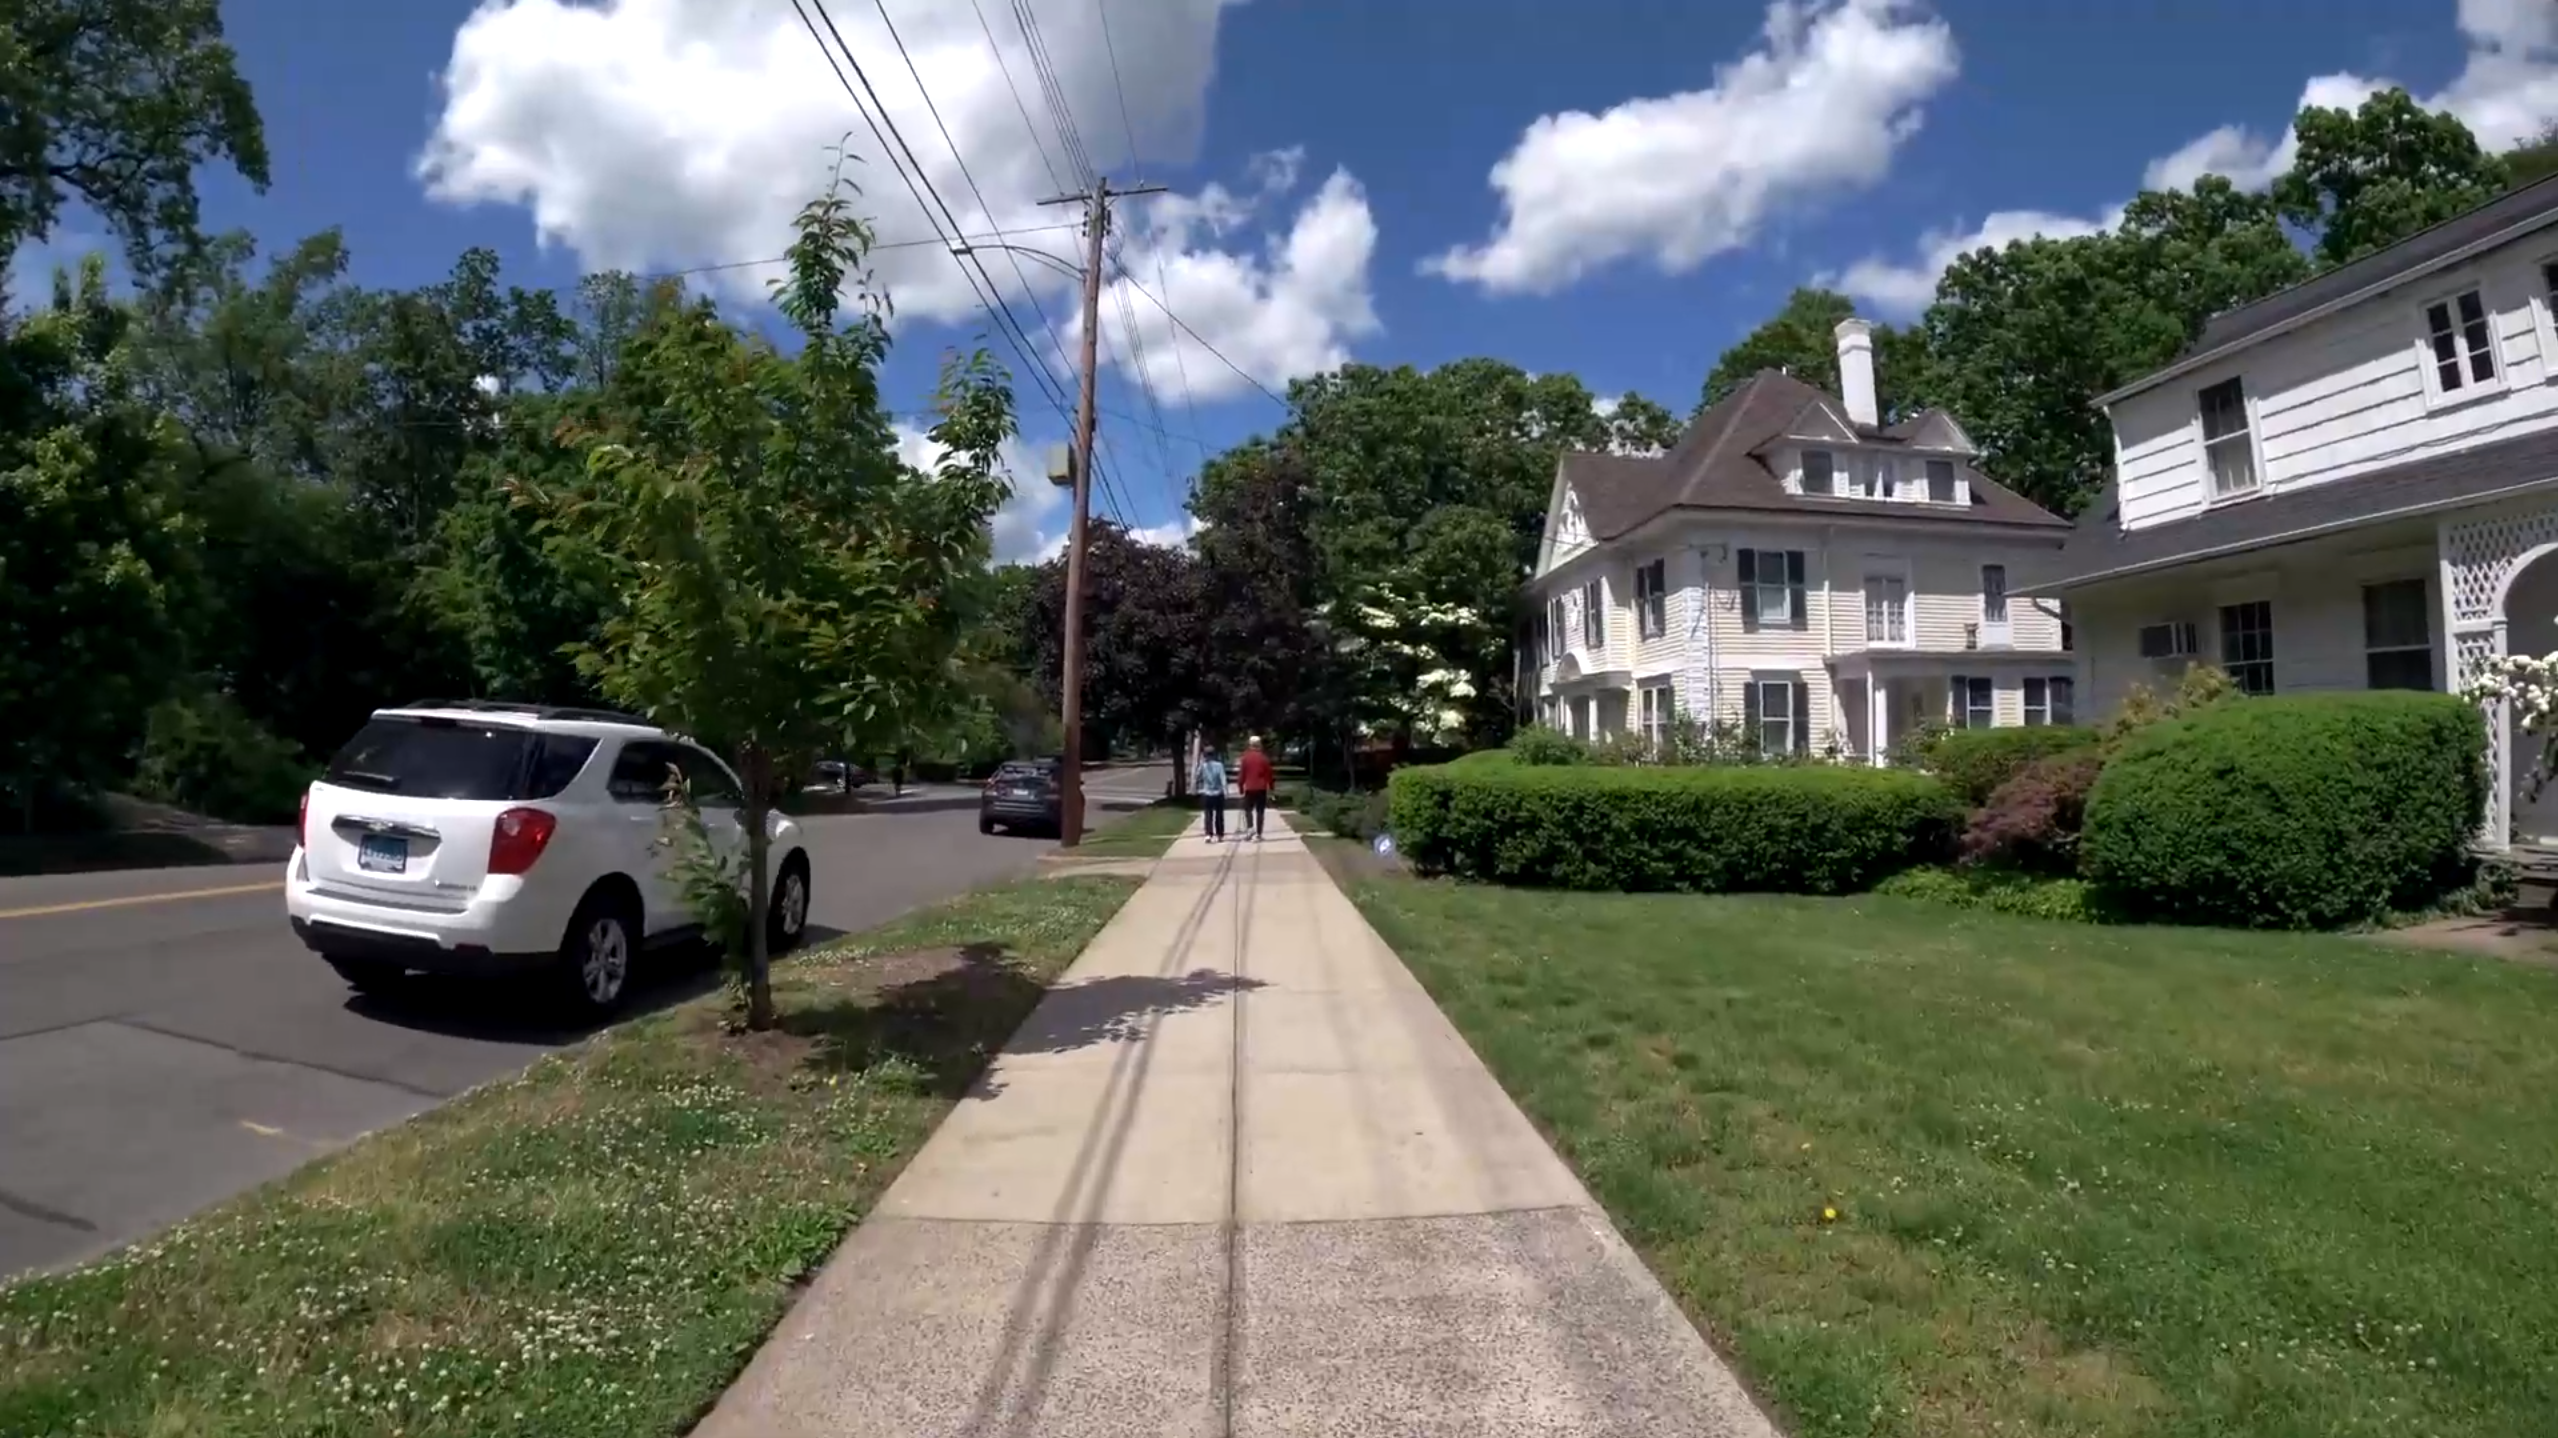
\includegraphics[width=0.80\textwidth]{screen_video_camminata}
\caption{Frame rappresentativo della sequenza di test: scena stradale con profondità prospettica, marciapiede convergente e oggetti a distanze variabili. Il movimento forward e le oscillazioni verticali legate ai passi costituiscono le perturbazioni principali da stabilizzare.}
\label{fig:screen_camminata}
\end{figure}

La scena presenta profondità prospettica con un marciapiede convergente, oggetti a distanze variabili e oscillazioni verticali ad alta frequenza sovrapposte al moto forward. Questo scenario è particolarmente adatto a evidenziare differenze tra modelli di trasformazione di complessità crescente.

Tutti i metodi sono stati eseguiti con \texttt{smoothing\_window}~=~45 e filtro gaussiano ($\sigma=2$), garantendo piena comparabilità dei risultati.

\section{Metriche di Valutazione}

Le prestazioni sono state misurate con:

\begin{itemize}
    \item \textbf{RMS} del moto incrementale su X, Y e rotazione (quantifica l'ampiezza del moto residuo),
    \item \textbf{Jitter Reduction (JR)} percentuale calcolata come riduzione della varianza degli step incrementali,
    \item \textbf{Tempo totale di elaborazione} (secondi, include solo i passaggi computazionali).
\end{itemize}

\[
RMS_x = \sqrt{\frac{1}{N-1}\sum_{t=2}^{N}(\Delta X_t)^2}, \qquad
JR_x = \left(1 - \frac{\mathrm{Var}(\Delta\tilde{X})}{\mathrm{Var}(\Delta X)}\right)\times 100\%
\]

\section{Risultati Quantitativi}

\begin{table}[H]
\centering
\begin{tabular}{lccccccc}
\toprule
Metodo & RMS X & RMS Y & RMS $\theta$ & JR X (\%) & JR Y (\%) & JR $\theta$ (\%) & Tempo (s) \\
\midrule
Block Matching        & \textbf{4.06} & \textbf{3.48} & --    & \textbf{97.4} & \textbf{94.9} & --    & 4843 \\
Opt.\ Partial         & 6.63 & 5.51 & 0.173 & 81.0 & 91.5 & 94.3 & 30.1 \\
Opt.\ Affine          & 6.53 & 5.85 & 0.173 & 84.5 & 90.8 & 95.8 & 30.1 \\
Opt.\ Homography      & 7.11 & 6.11 & 0.191 & 67.3 & 84.2 & 89.0 & 31.0 \\
ORB Partial           & \textbf{5.33} & 5.82 & 0.175 & 84.5 & \textbf{91.9} & 95.2 & 45.1 \\
ORB Affine            & 5.65 & 6.01 & 0.178 & 82.7 & 90.2 & 95.0 & 80.8 \\
ORB Homography        & 7.89 & 6.53 & 0.201 & 66.7 & 81.0 & 87.2 & 65.0 \\
\bottomrule
\end{tabular}
\caption{Confronto quantitativo tra tutti i metodi (\texttt{smoothing\_window}~=~45, filtro gaussiano $\sigma=2$). Block Matching non stima la componente rotazionale ($\theta$). In grassetto i valori migliori per ciascuna colonna (escluso Block Matching per il tempo, che impiega circa 4843\,s per via della ricerca esaustiva a grid)}
\label{tab:risultati}
\end{table}

\begin{figure}[H]
\centering
\includegraphics[width=\textwidth]{tabella_riepilogativa}
\caption{Tabella riepilogativa generata dall'interfaccia applicativa. I valori di Block Matching (JR~$>$~97\%) vanno letti con cautela: come mostrato dall'analisi delle traiettorie, il metodo stima moti nell'ordine di 100\,px cumulativi contro i $\sim$2500\,px di Optical Flow, indicando che il drift globale della camminata non viene stimato né compensato. Le metriche eccellenti di Block Matching riflettono la coerenza interna di una stima a corto raggio, non la qualità percettiva del video stabilizzato.}
\label{fig:tabella_riepilogativa}
\end{figure}

\section{Analisi delle Traiettorie}

Le figure seguenti mostrano le traiettorie cumulative lungo gli assi X e Y: la curva blu rappresenta il moto raw stimato frame per frame, mentre la curva arancione rappresenta il segnale filtrato (smoothed). La differenza tra le due curve è il contributo di compensazione applicato a ciascun frame.

\subsection{Block Matching}

\begin{figure}[H]
\centering
\includegraphics[width=0.9\textwidth]{traiettoria_block_matching}
\caption{Traiettorie cumulative X e Y -- Block Matching. I displacement massimi sono dell'ordine di 100\,px su X e 250\,px su Y: valori di gran lunga inferiori a quelli stimati dai metodi feature-based ($\sim$2500\,px su X per Optical Flow). Questo non indica maggiore stabilità, bensì la limitazione della ricerca a blocchi a corto raggio: il drift globale della camminata non viene catturato, e le metriche RMS/JR eccellenti riflettono la coerenza interna di una stima incompleta, non la qualità percettiva del video prodotto.}
\label{fig:traj_bm}
\end{figure}

\subsection{Optical Flow – Partial}

\begin{figure}[H]
\centering
\includegraphics[width=0.9\textwidth]{traiettoria_opt_partial}
\caption{Traiettorie cumulative X e Y -- Optical Flow Partial (Shi-Tomasi + LK). Il segnale filtrato insegue il drift forward lungo X preservando la stabilità verticale. Con RMS\,X~=~6.63\,px e JR\,Y~=~91.5\%, questo metodo offre il miglior compromesso tra qualità di stabilizzazione e velocità (30.1\,s).}
\label{fig:traj_opt_partial}
\end{figure}

\subsection{Optical Flow – Affine}

\begin{figure}[H]
\centering
\includegraphics[width=0.9\textwidth]{traiettoria_opt_affine}
\caption{Traiettorie cumulative X e Y -- Optical Flow Affine. Il modello affine introduce lieve miglioramento su JR\,X (84.5\% vs 81.0\% del Partial), ma incrementa RMS\,Y da 5.51 a 5.85\,px. La maggiore flessibilità del modello non si traduce in benefici sostanziali per questa tipologia di moto.}
\label{fig:traj_opt_affine}
\end{figure}

\subsection{Optical Flow – Homography}

\begin{figure}[H]
\centering
\includegraphics[width=0.9\textwidth]{traiettoria_opt_homo}
\caption{Traiettorie cumulative X e Y -- Optical Flow Homography. La traiettoria presenta oscillazioni più marcate rispetto al modello Partial: RMS\,X~=~7.11\,px e JR\,X~=~67.3\%, i valori più bassi tra le varianti Optical Flow. La proiettività amplifica gli outlier di matching in assenza di variazioni prospettiche reali.}
\label{fig:traj_opt_homo}
\end{figure}

\subsection{ORB Matching – Partial}

\begin{figure}[H]
\centering
\includegraphics[width=0.9\textwidth]{traiettoria_orb_partial}
\caption{Traiettorie cumulative X e Y -- ORB Partial. Il descrittore binario ORB consente una stima del moto traslazionale più precisa: RMS\,X~=~5.33\,px (il più basso tra i metodi feature-based) e JR\,Y~=~91.9\%. È il metodo a massima qualità tra quelli con tempi di elaborazione ragionevoli (45.1\,s).}
\label{fig:traj_orb_partial}
\end{figure}

\subsection{ORB Matching – Affine}

\begin{figure}[H]
\centering
\includegraphics[width=0.9\textwidth]{traiettoria_orb_affine}
\caption{Traiettorie cumulative X e Y -- ORB Affine. Il modello affine aumenta sensibilmente il tempo di elaborazione (80.8\,s, il più lento tra i metodi feature-based) senza migliorare le metriche rispetto a ORB Partial. RMS\,X~=~5.65\,px e JR\,X~=~82.7\% sono inferiori ai valori del modello Partial.}
\label{fig:traj_orb_affine}
\end{figure}

\subsection{ORB Matching – Homography}

\begin{figure}[H]
\centering
\includegraphics[width=0.9\textwidth]{traiettoria_orb_homo}
\caption{Traiettorie cumulative X e Y -- ORB Homography. La matrice omografica a 8 parametri produce i risultati peggiori nella famiglia ORB: RMS\,X~=~7.89\,px e JR\,X~=~66.7\%. Il matching ORB con omografia è particolarmente suscettibile agli outlier proiettivi in scene planari con moto prevalentemente traslazionale.}
\label{fig:traj_orb_homo}
\end{figure}

\section{Grafici Comparativi}

\begin{figure}[H]
\centering
\includegraphics[width=\textwidth]{grafici_comparativi_1}
\caption{Grafici comparativi (Parte~1): confronto tra metodi per RMS\,X, RMS\,Y e RMS\,$\theta$. I valori di Block Matching ($\approx$4\,px su X, $\approx$3.5\,px su Y) appaiono i migliori in assoluto, ma questo dato va interpretato con cautela: come evidenziato dall'analisi delle traiettorie (Figure~\ref{fig:traj_bm} e~\ref{fig:traj_opt_partial}), Block Matching stima un moto cumulativo di soli $\sim$100\,px contro i $\sim$2500\,px di Optical Flow. Le metriche RMS eccellenti riflettono dunque la \emph{scala ridotta} del moto stimato, non la qualità del video prodotto. I valori dei metodi feature-based (Optical e ORB) sono invece comparabili tra loro e rappresentano una misura affidabile del jitter residuo reale.}
\label{fig:grafici_comp_1}
\end{figure}

\begin{figure}[H]
\centering
\includegraphics[width=\textwidth]{grafici_comparativi_2}
\caption{Grafici comparativi (Parte~2): confronto tra metodi per Jitter Reduction percentuale su X, Y e $\theta$, e tempo di elaborazione. La JR di Block Matching ($>$97\%) è concettualmente non confrontabile con quella dei metodi feature-based: Block Matching riduce quasi interamente il poco moto che riesce a stimare, ma lascia il drift globale della camminata invariato, producendo un video percettivamente instabile. Il confronto significativo è quindi solo tra i metodi feature-based: ORB Partial e Optical Partial/Affine guidano con JR $>$80\% su entrambi gli assi, mentre le varianti Homography risultano sistematicamente inferiori. Sul piano del tempo, Block Matching è fuori scala ($\approx$4843\,s); tra i metodi feature-based Optical (30\,s) è circa il 50\% più veloce di ORB (45--81\,s).}
\label{fig:grafici_comp_2}
\end{figure}

\section{Discussione dei Risultati}

\subsection{Limiti delle metriche quantitative: il caso Block Matching}

Un confronto diretto tra le traiettorie di Block Matching e Optical Flow rivela una differenza concettuale fondamentale che le sole metriche numeriche non catturano.

La traiettoria di \textbf{Block Matching} (Figura~\ref{fig:traj_bm}) mostra un displacement cumulativo massimo di circa 100\,px su X e 250\,px su Y. La curva raw presenta oscillazioni visibili attorno alla tendenza generale, e la curva smoothed le segue con profilo attenuato -- le due curve sono distinguibili ma entrambe rimangono confinate in un range di spostamento molto limitato rispetto ai metodi feature-based. La traiettoria di \textbf{Optical Flow Partial} (Figura~\ref{fig:traj_opt_partial}), invece, raggiunge circa $-2500$\,px su X e $-800$\,px su Y: lo smoothing segue fedelmente il drift globale rimuovendo le oscillazioni ad alta frequenza.

Questa differenza non riflette una maggiore stabilità del video prodotto da Block Matching, bensì una \textbf{stima del moto incompleta}: la ricerca a blocchi opera su una finestra di ricerca limitata e stima solo traslazioni intere a corto raggio, rendendo invisibile il drift cumulativo della camminata. Di conseguenza:

\begin{itemize}
    \item il valore RMS calcolato è basso perché gli spostamenti stimati sono piccoli \emph{per costruzione}, non perché il video sia più stabile,
    \item la JR del 97\% rappresenta la riduzione del poco jitter che il metodo riesce a stimare, lasciando il moto globale sostanzialmente non compensato,
    \item il risultato visivo è un video che mantiene il drift della camminata, percepito dall'occhio umano come instabilità residua.
\end{itemize}

Optical Flow, stimando la traiettoria cumulativa reale, permette allo smoothing di applicare una compensazione ampia e continua. Il video stabilizzato risulta \textbf{percettivamente molto più stabile} nonostante le metriche numeriche (RMS e JR) siano inferiori a quelle di Block Matching.

Questo caso evidenzia un limite intrinseco delle metriche basate sul moto stimato: esse misurano la coerenza interna della stima, non la qualità percettiva della stabilizzazione. Un metodo che sottostima sistematicamente il moto reale può ottenere metriche eccellenti pur producendo un output visivamente inferiore.

\subsection{Optical Flow vs ORB}

A parità di modello di trasformazione (Partial), ORB fornisce un RMS\,X inferiore (5.33 vs 6.63\,px), confermando una stima del moto di base più precisa grazie ai descrittori binari. Optical Flow è invece più veloce (30.1 vs 45.1\,s), con un vantaggio di circa il 50\% sul tempo.

Per JR\,Y i due metodi sono sostanzialmente equivalenti (91.9\% vs 91.5\%), mentre ORB Partial supera Optical Partial su JR\,X (84.5\% vs 81.0\%).

La scelta tra le due famiglie dipende quindi dal vincolo applicativo: Optical Partial per il miglior compromesso qualità/tempo, ORB Partial per la massima stabilità. Entrambi stimano correttamente il moto globale cumulativo, garantendo una compensazione percettivamente efficace.

\subsection{Confronto tra Modelli di Trasformazione}

All'interno di entrambe le famiglie algoritmiche, il trend è coerente:

\begin{itemize}
    \item Partial $\geq$ Affine $>$ Homography in termini di JR e RMS,
    \item il tempo di elaborazione cresce con la complessità del modello,
    \item l'Homography penalizza sistematicamente le prestazioni di stabilizzazione.
\end{itemize}

Il modello Affine introduce parametri di scala differenziale e shear non necessari per descrivere le oscillazioni di camminata, risultando marginalmente peggiore rispetto al Partial. Il modello Homography (8 parametri) è chiaramente sovra-parametrizzato: amplifica gli outlier di matching proiettando errori locali in deformazioni geometriche globali (RMS\,X~=~7.89\,px per ORB Homography).

\subsection{Considerazioni sulla Sovra-Parametrizzazione}

I risultati confermano un principio generale: la complessità del modello deve essere commisurata alla natura del moto. Per una sequenza con moto forward costante e oscillazioni verticali periodiche, un modello a 4 parametri (traslazione + rotazione + scala isotropa) cattura il moto rilevante senza introdurre gradi di libertà instabili.

\section{Sintesi e Verdetto}

Escludendo Block Matching — le cui metriche numeriche eccellenti sono un artefatto della stima incompleta del moto, non una misura di qualità percettiva — \textbf{l'algoritmo migliore in assoluto per questa sequenza è ORB Partial}, con il miglior RMS\,X tra i metodi feature-based (5.33\,px) e la JR più alta su entrambi gli assi (84.5\% / 91.9\%) a fronte di un tempo di elaborazione accettabile (45.1\,s).

Se il vincolo è il tempo, \textbf{Optical Partial} rappresenta la scelta ottimale: produce una stabilità percettiva pressoché equivalente (JR 81.0\% / 91.5\%) in soli 30.1\,s, con un risparmio del 33\% rispetto a ORB Partial.

\begin{itemize}
    \item \textbf{Algoritmo migliore (qualità)}: \textbf{ORB Partial} — massima stabilità percettiva, stima del moto globale precisa, JR\,Y~=~91.9\%.
    \item \textbf{Algoritmo migliore (qualità/velocità)}: \textbf{Optical Partial} — risultato visivo equivalente a ORB Partial, 30.1\,s di elaborazione.
    \item \textbf{Da evitare}: varianti Homography (sovra-parametrizzazione, JR\,X $\leq$ 67\%) e Block Matching (stima del moto incompleta, risultato visivo inferiore nonostante JR numerica $>$97\%).
\end{itemize}

La lezione principale è che le metriche basate sulla stima del moto non sono sufficienti a valutare la qualità percettiva: occorre tenere conto della completezza della stima (copertura del moto reale) e non solo della sua coerenza interna.
